\chapter{Theoretische Achtergrond}
\label{hst-theorie}
Dit hoofdstuk bevat de theoretische concepten die nodig zijn om de gebruikte aanpak zo goed mogelijk te begrijpen. Het bevat een beschrijving van de gebruikte neurale netwerken en van een aantal concepten uit de statistiek.

\section{Recurrente Neurale Netwerken}
Recurrente neurale netwerken zijn een uitbreiding van standaard feedforward neurale netwerken. Ze kunnen, net zoals feedforward netwerken, getraind worden met terugpropagatie. Het grote verschil met feedforward netwerken is dat de output van de vorige stap wordt teruggekoppeld naar de verborgen layers. Op figuur \ref{fig:rnn} is te zien hoe een RNN ontrold wordt over de verschillende tijdstippen. Dit zorgt ervoor dat het netwerk in staat is om dingen te onthouden. Hierdoor kunnen recurrente netwerken zeer goed om met het coderen van tijdsgerelateerde informatie. Dit is zeer geschikt om sequenti\"ele data, zoals tekst, te voorspellen. Recurrente neurale netwerken kunnen bijgevolg gebruikt worden als een language model.\

\begin{figure}[tb]
    \centering
    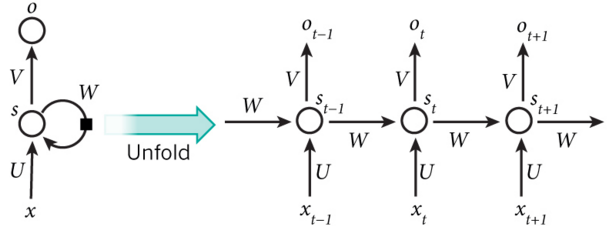
\includegraphics[width=\linewidth]{Images/rnn.PNG}
    \label{fig:rnn}
    \caption{Ontrolling van een recurrent neuraal netwerk}
\end{figure}

Het voorspellen van een zin met een RNN gebeurt woord per woord. Op basis van de eerder waargenomen woorden kan een voorspelling gemaakt worden van het volgende woord. De woorden worden in de vorm van vectorrepresentaties aan het netwerk gegeven. Deze encodering kan gebruik maken van one-hot codering, ze kan random zijn, of er kan gebruik gemaakt worden van word embeddings zoals bijvoorbeeld \emph{word2vec}\cite{Mikolov2013}.
\section{Convolutionele Neurale Netwerken}

\section{Long Short Term Memory Neurale Netwerken}
Long Short Term Memory (LSTM) is een vorm van RNN die geheugencellen bevat. Door deze cellen is het netwerk in staat om op lange termijn informatie over de input bij te houden. Elk LSTM blok heeft een aantal gates om te bepalen of de input moet onthouden worden, en of een vorige waarde moet bijgehouden of vergeten worden. De output van de cellen is bijgevolg afhankelijk van alle eerder geobserveerde inputs. Op figuur \ref{fig:lstm} is te zien hoe een LSTM-blok er uitziet.\cite{Google}\cite{SeppHochreiter1997}

\begin{figure}[tb]
    \centering
    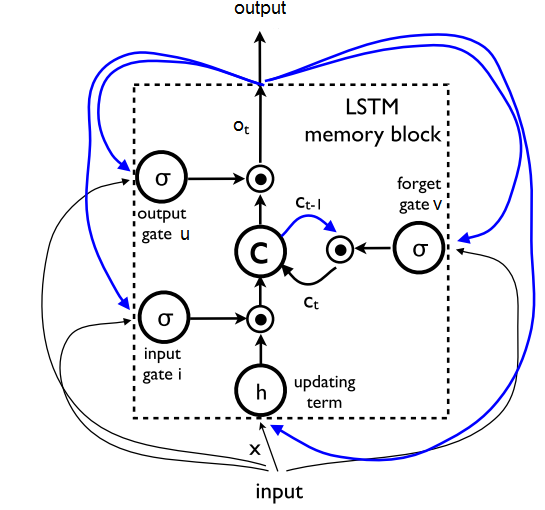
\includegraphics[width=\linewidth]{Images/lstm.PNG}
    \label{fig:lstm}
    \caption{Long Short Term Memory geheugenblok}
\end{figure}

LSTM netwerken worden net als RNN gebruikt als language models en zorgen over het algemeen voor hogere kwaliteit. Dit komt doordat LSTM netwerken een langere periode hebben waarover de input kan onthouden worden. Door het geheugen dat langer kan onthouden dan een RNN is het mogelijk om sequenties met een langere periode tussen belangrijke events te modelleren. 
\section{Latent Dirichlet Allocation}
Latent Dirichlet Allocation is een generatief probabilistisch model voor dsicrete data. Een van de meest gebruikte toepassingen hiervan is het modelleren van een een verdeling van onderwerpen in een set van tekstdocumenten. Dit conecpt is gebaseerd op de veronderstelling dat elk document een zeker kansverdeling heeft over alle mogelijke onderwerpen. Deze onderwerpen hebben dan een kansverdeling over alle mogelijke woorden. Zo kan de kans dat een bepaald document $d_j$ een bepaald woord $w_i$ bevat worden geschreven als een som over alle verschillende topics (formule \ref{formule:lda}). 

\begin{equation}
    \label{formule:lda}
    P(w_i | d_j) = \sum\limits_{k=0}^{n_{topics}}P(w_i|topic_k)P(topic_k|d_j)
\end{equation}

Het generatieve aspect van LDA is te zien in figuur \ref{fig:lda}. Op basis van twee Dirichlet priors $\alpha$ en $\beta$ word een kansverdeling over de onderwerpen gesampled per document ($\theta$), alsook een kansverdeling over de woorden voor elk onderwerp ($\phi$). Uit $\theta$ wordt voor elke positie $i$ in een document $j$ een onderwerp gesampled ($z_{ji}$). Het samplen van de woordverdeling voor dit onderwerp leidt tot het woord $w_{ji}$. Trainen van een LDA model gebeurt bijvoorbeeld met Gibbs sampling, en leidt tot de verdelingen $\theta$ en $\phi$.

\begin{figure}[tb]
    \centering
    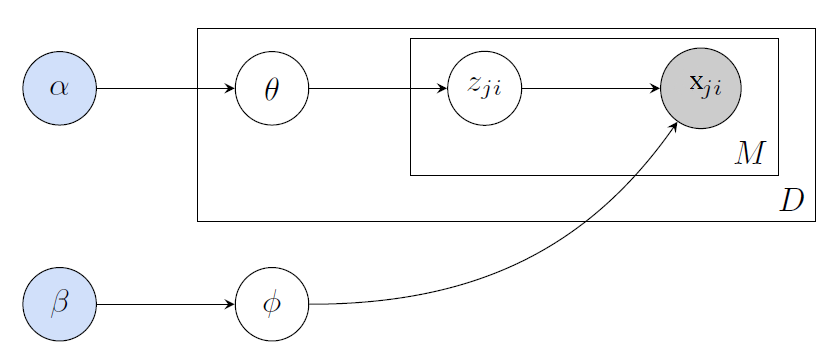
\includegraphics[width=\linewidth]{Images/lda.png}
    \label{fig:lda}
    \caption{Grafische weergave van LDA}
\end{figure}

\section{Stacked Canonical Correlation Analysis}
